\PassOptionsToPackage{unicode=true}{hyperref} % options for packages loaded elsewhere
\PassOptionsToPackage{hyphens}{url}
%
\documentclass[]{article}
\usepackage{lmodern}
\usepackage{amssymb,amsmath}
\usepackage{ifxetex,ifluatex}
\usepackage{fixltx2e} % provides \textsubscript
\ifnum 0\ifxetex 1\fi\ifluatex 1\fi=0 % if pdftex
  \usepackage[T1]{fontenc}
  \usepackage[utf8]{inputenc}
  \usepackage{textcomp} % provides euro and other symbols
\else % if luatex or xelatex
  \usepackage{unicode-math}
  \defaultfontfeatures{Ligatures=TeX,Scale=MatchLowercase}
\fi
% use upquote if available, for straight quotes in verbatim environments
\IfFileExists{upquote.sty}{\usepackage{upquote}}{}
% use microtype if available
\IfFileExists{microtype.sty}{%
\usepackage[]{microtype}
\UseMicrotypeSet[protrusion]{basicmath} % disable protrusion for tt fonts
}{}
\IfFileExists{parskip.sty}{%
\usepackage{parskip}
}{% else
\setlength{\parindent}{0pt}
\setlength{\parskip}{6pt plus 2pt minus 1pt}
}
\usepackage{hyperref}
\hypersetup{
            pdfborder={0 0 0},
            breaklinks=true}
\urlstyle{same}  % don't use monospace font for urls
\usepackage[left=2cm,right=2cm,top=1cm,bottom=2cm]{geometry}
\usepackage{color}
\usepackage{fancyvrb}
\newcommand{\VerbBar}{|}
\newcommand{\VERB}{\Verb[commandchars=\\\{\}]}
\DefineVerbatimEnvironment{Highlighting}{Verbatim}{commandchars=\\\{\}}
% Add ',fontsize=\small' for more characters per line
\newenvironment{Shaded}{}{}
\newcommand{\AlertTok}[1]{\textcolor[rgb]{1.00,0.00,0.00}{\textbf{#1}}}
\newcommand{\AnnotationTok}[1]{\textcolor[rgb]{0.38,0.63,0.69}{\textbf{\textit{#1}}}}
\newcommand{\AttributeTok}[1]{\textcolor[rgb]{0.49,0.56,0.16}{#1}}
\newcommand{\BaseNTok}[1]{\textcolor[rgb]{0.25,0.63,0.44}{#1}}
\newcommand{\BuiltInTok}[1]{#1}
\newcommand{\CharTok}[1]{\textcolor[rgb]{0.25,0.44,0.63}{#1}}
\newcommand{\CommentTok}[1]{\textcolor[rgb]{0.38,0.63,0.69}{\textit{#1}}}
\newcommand{\CommentVarTok}[1]{\textcolor[rgb]{0.38,0.63,0.69}{\textbf{\textit{#1}}}}
\newcommand{\ConstantTok}[1]{\textcolor[rgb]{0.53,0.00,0.00}{#1}}
\newcommand{\ControlFlowTok}[1]{\textcolor[rgb]{0.00,0.44,0.13}{\textbf{#1}}}
\newcommand{\DataTypeTok}[1]{\textcolor[rgb]{0.56,0.13,0.00}{#1}}
\newcommand{\DecValTok}[1]{\textcolor[rgb]{0.25,0.63,0.44}{#1}}
\newcommand{\DocumentationTok}[1]{\textcolor[rgb]{0.73,0.13,0.13}{\textit{#1}}}
\newcommand{\ErrorTok}[1]{\textcolor[rgb]{1.00,0.00,0.00}{\textbf{#1}}}
\newcommand{\ExtensionTok}[1]{#1}
\newcommand{\FloatTok}[1]{\textcolor[rgb]{0.25,0.63,0.44}{#1}}
\newcommand{\FunctionTok}[1]{\textcolor[rgb]{0.02,0.16,0.49}{#1}}
\newcommand{\ImportTok}[1]{#1}
\newcommand{\InformationTok}[1]{\textcolor[rgb]{0.38,0.63,0.69}{\textbf{\textit{#1}}}}
\newcommand{\KeywordTok}[1]{\textcolor[rgb]{0.00,0.44,0.13}{\textbf{#1}}}
\newcommand{\NormalTok}[1]{#1}
\newcommand{\OperatorTok}[1]{\textcolor[rgb]{0.40,0.40,0.40}{#1}}
\newcommand{\OtherTok}[1]{\textcolor[rgb]{0.00,0.44,0.13}{#1}}
\newcommand{\PreprocessorTok}[1]{\textcolor[rgb]{0.74,0.48,0.00}{#1}}
\newcommand{\RegionMarkerTok}[1]{#1}
\newcommand{\SpecialCharTok}[1]{\textcolor[rgb]{0.25,0.44,0.63}{#1}}
\newcommand{\SpecialStringTok}[1]{\textcolor[rgb]{0.73,0.40,0.53}{#1}}
\newcommand{\StringTok}[1]{\textcolor[rgb]{0.25,0.44,0.63}{#1}}
\newcommand{\VariableTok}[1]{\textcolor[rgb]{0.10,0.09,0.49}{#1}}
\newcommand{\VerbatimStringTok}[1]{\textcolor[rgb]{0.25,0.44,0.63}{#1}}
\newcommand{\WarningTok}[1]{\textcolor[rgb]{0.38,0.63,0.69}{\textbf{\textit{#1}}}}
\usepackage{graphicx,grffile}
\makeatletter
\def\maxwidth{\ifdim\Gin@nat@width>\linewidth\linewidth\else\Gin@nat@width\fi}
\def\maxheight{\ifdim\Gin@nat@height>\textheight\textheight\else\Gin@nat@height\fi}
\makeatother
% Scale images if necessary, so that they will not overflow the page
% margins by default, and it is still possible to overwrite the defaults
% using explicit options in \includegraphics[width, height, ...]{}
\setkeys{Gin}{width=\maxwidth,height=\maxheight,keepaspectratio}
\setlength{\emergencystretch}{3em}  % prevent overfull lines
\providecommand{\tightlist}{%
  \setlength{\itemsep}{0pt}\setlength{\parskip}{0pt}}
\setcounter{secnumdepth}{0}
% Redefines (sub)paragraphs to behave more like sections
\ifx\paragraph\undefined\else
\let\oldparagraph\paragraph
\renewcommand{\paragraph}[1]{\oldparagraph{#1}\mbox{}}
\fi
\ifx\subparagraph\undefined\else
\let\oldsubparagraph\subparagraph
\renewcommand{\subparagraph}[1]{\oldsubparagraph{#1}\mbox{}}
\fi

% set default figure placement to htbp
\makeatletter
\def\fps@figure{htbp}
\makeatother


\date{}

\begin{document}

\hypertarget{requisiti-ristrutturati}{%
\section{\texorpdfstring{\texttt{Requisiti\ ristrutturati}}{Requisiti ristrutturati}}\label{requisiti-ristrutturati}}

Questa base di dati dovra' svolgere diverse mansioni anche motlo diverse
fra di loro, ovvero:

\hypertarget{organizzare-i-prodotti-in-inventario}{%
\paragraph{\texorpdfstring{\texttt{Organizzare\ i\ prodotti\ in\ inventario}}{Organizzare i prodotti in inventario}}\label{organizzare-i-prodotti-in-inventario}}

in modo da avere quanta piu' automazione possibile, quindi, per esempio,
sapere quando un prodotto sta per finire, aggiornare in automatico le
quantita' di un dato prodotto quando questo viene acquistato da un
cliente oppure rifornito tramite donazione o acquisto del market,
effettuare lo scarico dei prodotti molto vicini alla data di scadenza e
memorizzare ogni ingresso prodotti nel market. Il market puo' inoltre
acquistare dei prodotti in autonomia nel caso in cui, per esempio, un
dato prodotto non venga donato.

\textbf{Per ogni prodotto}, si memorizzano la marca, il prezzo in punti,
la data di scadenza (\underline{nel caso di beni deperibili}) e la data
di scadenza ``reale'', ovvero la data (dopo la data di scadenza) in cui
un dato prodotto non e' piu' utilizzabile/commestibile.

\textbf{Per ogni scorta di prodotti} viene salvata la tiplogia del
prodotto (shampoo, tonno, pasta\ldots{}), la marca (Garnier, Rio Mare,
Barilla\ldots{}) e la relativa quantita' disponibile.

\textbf{Per ogni ingresso prodotti} viene salvata la data e l'ora

\textbf{Per ogni scarico prodotti} viene salvata la data e l'ora.

\underline{NOTA}: supponiamo che per ogni scarico si definiscano la data
e l'ora, ma che il volontario gli venga assegnato in seguito perche',
per esempio, lo scarico e' tra un mese.

\hypertarget{gestire-i-vari-appuntamenti-con-la-clientela}{%
\paragraph{\texorpdfstring{\texttt{Gestire\ i\ vari\ appuntamenti\ con\ la\ clientela}}{Gestire i vari appuntamenti con la clientela}}\label{gestire-i-vari-appuntamenti-con-la-clientela}}

in modo da memorizzare i vari dati di un appuntamento oltre a poter
risalire al cliente che vi ha partecipato, al volontario che lo ha
supervisioanto a quali prodotti sono stati acquistati. E' inoltre
necessario risalire non solo al cliente ma anche al suo nucleo
familiare, siccome i suoi componenti possono acquistare i prodotti a
nome del cliente stesso (\underline{se autorizzati a spendere i punti},
in genere chi e' sopra i 16 anni d'eta'). Supponiamo che un cliente
possa avere piu' contatti (recapiti telefonici e email) e che fornisca
lui i recapiti dei familiari, di conseguenza i familiari non dovranno
fornire alcun recapito.

\textbf{Per ogni appuntamento} si memorizza la data, l'ora, il
componente del nucleo familiare che vi prende parte, il saldo iniziale e
il saldo finale.

\hypertarget{ricevere-le-donazioni}{%
\subparagraph{\texorpdfstring{\texttt{Ricevere\ le\ donazioni}}{Ricevere le donazioni}}\label{ricevere-le-donazioni}}

che possono essere in denaro oppure prodotti, forniti da diverse
tipolgie di donatori (privati, negozi, associazioni). Nel caso delle
donazioni in prodotti, la consegna al market viene effettuata
rispettivamente dal privato nel caso appunto di una donazione in
prodotti da un privato, e da un volontario se invece la donazione e'
fatta da un negozio o associazione. In ogni caso, ogni donazione viene
salvata e collegata al suo donatore e nel caso di una donazione in
denaro verra' salvato l'importo, mentre per la donazione in prodotti
verra' aggiornato l'inventario e verra' salvato l'ingresso prodotti.

\textbf{Per ogni donazione} vengono memorizzate la data, l'ora, e, nel
caso di una donazione in denaro, l'importo,

\textbf{Per ogni donatore} vengono memorizzati i recapiti (numero di
telefono e email), univoci per ogni donatore. Nel caso di un donatore
privato si salvano inoltre il nome, il cognome, la data di nascita e il
codice fiscale. Per i negozi si salva la ragione sociale e la partita
IVA e, infine, per le associazioni il nome e il codice fiscale.

\hypertarget{organizzare-il-lavoro-dei-volontari}{%
\paragraph{\texorpdfstring{\texttt{Organizzare\ il\ lavoro\ dei\ volontari}}{Organizzare il lavoro dei volontari}}\label{organizzare-il-lavoro-dei-volontari}}

memorizzando per quali servizi un dato volontario e' disponibile (e in
quali giorni/ore) e organizzando i turni anche in base a queste
informazioni.

\textbf{Per ogni volontario} si salva il nome, il cognome, la data di
nascita, le (eventuali) associazioni a cui e' collegato e i recapiti
(univoci, email e numero di telefono).

\textbf{Per ogni turno} si salva la data, l'ora di inizio e l'ora di
fine. Nel caso di un turno di trasporto merci, si salva anche l'ora del
trasporto, il numero di colli da trasportare e la sede del ritiro.

\textbf{Per ogni servizio} vengono salvati il nome (es. ritiro merci) e,
nel caso di un trasporto merci, il tipo di veicolo utilizzato.

\hypertarget{progetto-concettuale}{%
\subsection{\texorpdfstring{\texttt{Progetto\ concettuale}}{Progetto concettuale}}\label{progetto-concettuale}}

\begin{figure}
\centering
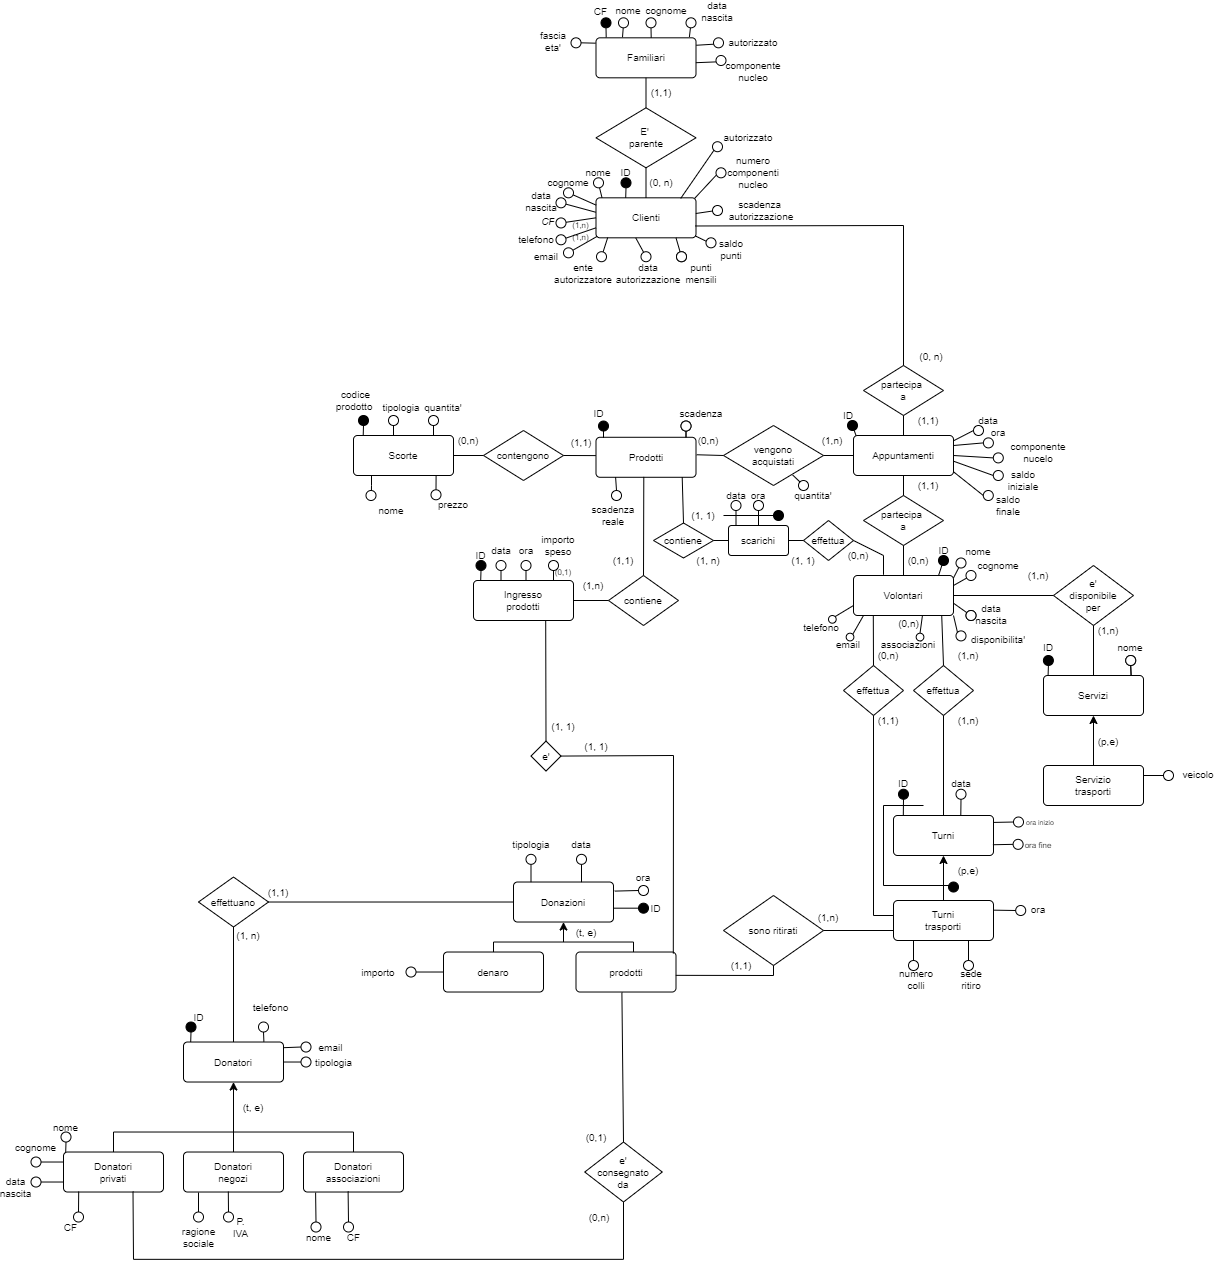
\includegraphics{media/social_market_v2.drawio.png}
\caption{Diagramma ER}
\end{figure}

\begin{figure}
\centering
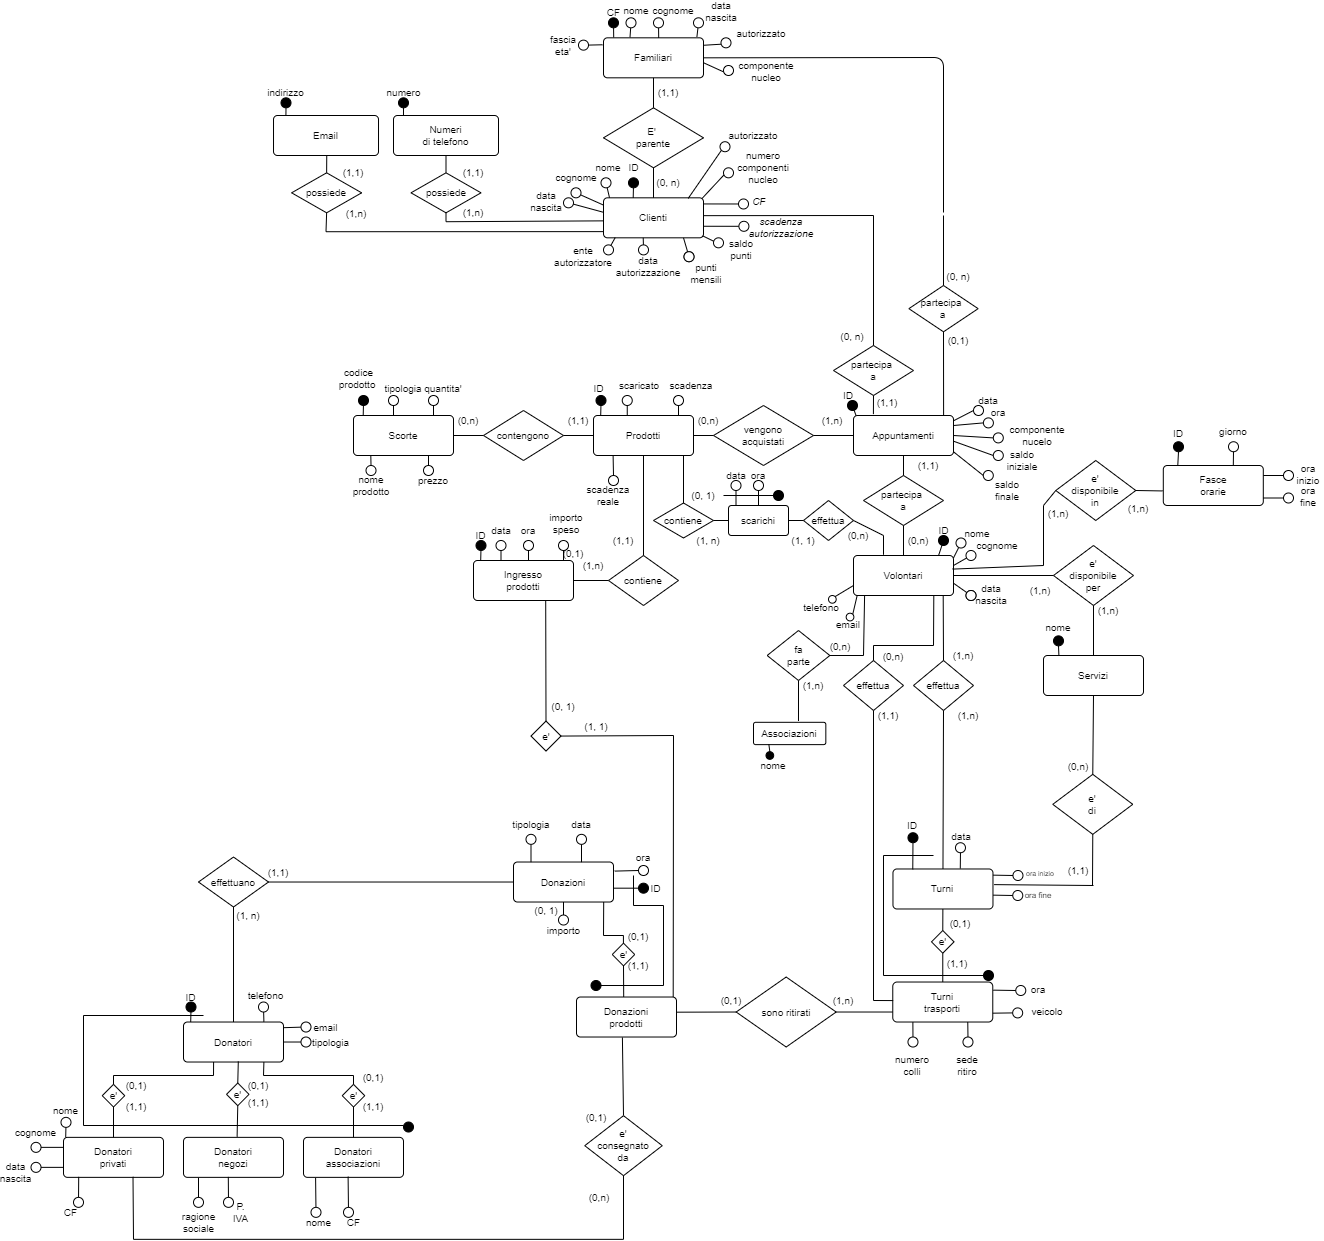
\includegraphics{media/social_market_v2_ristrutturato.drawio.png}
\caption{Diagramma ER ristrutturato}
\end{figure}

\newpage

\hypertarget{dizionario-entita}{%
\subsection{\texorpdfstring{\texttt{Dizionario\ entita\textquotesingle{}}}{Dizionario entita'}}\label{dizionario-entita}}

\begin{itemize}
\item
  \texttt{Telefoni}

  \begin{itemize}
  \tightlist
  \item
    \textbf{numero}: \texttt{string}
  \item
    cliente\(^{clienti}\): \texttt{int}

    \begin{itemize}
    \tightlist
    \item
      identificativo del cliente a cui e' collegato il numero di
      telefono
    \end{itemize}
  \end{itemize}
\item
  \texttt{Email}

  \begin{itemize}
  \tightlist
  \item
    \textbf{indirizzo}: \texttt{string}
  \item
    cliente\(^{clienti}\): \texttt{int}

    \begin{itemize}
    \tightlist
    \item
      identificativo del cliente a cui e' collegato l'indirizzo email
    \end{itemize}
  \end{itemize}
\item
  \texttt{Clienti}

  \begin{itemize}
  \tightlist
  \item
    \textbf{ID}: \texttt{int}

    \begin{itemize}
    \tightlist
    \item
      Numero identificativo (unico per ogni cliente)
    \end{itemize}
  \item
    nome: \texttt{string}
  \item
    cognome: \texttt{string}
  \item
    data di nascita: \texttt{date}
  \item
    codice fiscale: \texttt{string}
  \item
    ente\_autorizzatore: \texttt{string}

    \begin{itemize}
    \tightlist
    \item
      L'ente che ha concesso l'autorizzazione al cliente
    \end{itemize}
  \item
    data\_autorizzazione: \texttt{date}

    \begin{itemize}
    \tightlist
    \item
      data di conseguimento dell'autorizzazione
    \end{itemize}
  \item
    scadenza\_autorizzazione: \texttt{date}

    \begin{itemize}
    \tightlist
    \item
      di default dopo 6 mesi dalla data di autorizzazione
    \end{itemize}
  \item
    punti\_mensili: \texttt{int}

    \begin{itemize}
    \tightlist
    \item
      saldo mensile che ogni cliente puo' spendere
    \end{itemize}
  \item
    saldo\_punti: \texttt{int}

    \begin{itemize}
    \tightlist
    \item
      saldo punti attuale
    \end{itemize}
  \item
    n\_componenti\_nucleo: \texttt{int}

    \begin{itemize}
    \tightlist
    \item
      il numero dei componenti del nucleo familiare
    \end{itemize}
  \item
    autorizzato: \texttt{bool}

    \begin{itemize}
    \tightlist
    \item
      se il cliente e' autorizzato a spendere i punti oppure no
    \end{itemize}
  \end{itemize}
\item
  \texttt{Familiari}

  \begin{itemize}
  \tightlist
  \item
    \textbf{CF}: \texttt{string}

    \begin{itemize}
    \tightlist
    \item
      codice fiscale
    \end{itemize}
  \item
    nome: \texttt{string}
  \item
    cognome: \texttt{string}
  \item
    data\_nascita: \texttt{date}
  \item
    componente\_nucleo: \texttt{string}

    \begin{itemize}
    \tightlist
    \item
      quale componente del nucleo familiare e' (padre, madre,
      figlio\ldots{})
    \end{itemize}
  \item
    autorizzato: \texttt{bool}

    \begin{itemize}
    \tightlist
    \item
      se e' autorizzato a spendere i punti oppure no
    \end{itemize}
  \end{itemize}
\item
  \texttt{Volontari}

  \begin{itemize}
  \tightlist
  \item
    \textbf{ID}: \texttt{int}

    \begin{itemize}
    \tightlist
    \item
      Numero identificativo del volontario (unico per ogni volontario)
    \end{itemize}
  \item
    nome: \texttt{string}
  \item
    cognome: \texttt{string}
  \item
    data di nascita: \texttt{date}
  \item
    telefono: \texttt{string}

    \begin{itemize}
    \tightlist
    \item
      unico per ogni volontario
    \end{itemize}
  \item
    email: \texttt{string}

    \begin{itemize}
    \tightlist
    \item
      unico per ogni volontario
    \end{itemize}
  \item
    disponibilita': \texttt{string}

    \begin{itemize}
    \tightlist
    \item
      fascia oraria e giorni in cui e' disponibile per i servizi (es. il
      giovedi' dalle 3 alle 5)
    \end{itemize}
  \end{itemize}
\item
  \texttt{Associazioni}

  \begin{itemize}
  \tightlist
  \item
    \textbf{nome}: \texttt{string}
  \end{itemize}
\item
  \texttt{Prodotti}

  \begin{itemize}
  \tightlist
  \item
    \textbf{ID}: \texttt{int}

    \begin{itemize}
    \tightlist
    \item
      identificativo del singolo prodotto
    \end{itemize}
  \item
    scadenza: \texttt{date}
  \item
    scadenza\_reale: \texttt{date}

    \begin{itemize}
    \tightlist
    \item
      data oltre il quale e' necessario effettuare lo scarico del
      prodotto
    \end{itemize}
  \item
    codice\_prodotto\(^{scorte}\): \texttt{int}

    \begin{itemize}
    \tightlist
    \item
      identificativo della categoria di prodotto
    \end{itemize}
  \item
    ID\_ingresso\(^{ingresso\_prodotti}\): \texttt{int}

    \begin{itemize}
    \tightlist
    \item
      ingresso prodotti in cui il singolo prodotto e' entrato nel market
    \end{itemize}
  \item
    data\_scarico\(^{scarichi}\): \texttt{date}
  \item
    ora\_scarico\(^{scarichi}\): \texttt{time}
  \end{itemize}
\item
  \texttt{Scarichi}

  \begin{itemize}
  \tightlist
  \item
    \textbf{data}: \texttt{date}
  \item
    \textbf{ora}: \texttt{time}
  \item
    volontario\(^{volontari}\): \texttt{int}
  \end{itemize}
\item
  \texttt{Scorte}

  \begin{itemize}
  \tightlist
  \item
    \textbf{codice\_prodotto}: \texttt{int}

    \begin{itemize}
    \tightlist
    \item
      codice identificativo per tutti i prodotti con una data tipologia
      e marca
    \end{itemize}
  \item
    tipologia: \texttt{string}

    \begin{itemize}
    \tightlist
    \item
      Tipologia generica del prodotto (pasta, tonno\ldots{})
    \end{itemize}
  \item
    marca: \texttt{string}

    \begin{itemize}
    \tightlist
    \item
      marca del prodotto (de Cecco, Rio Mare\ldots{})
    \end{itemize}
  \item
    prezzo: \texttt{float}

    \begin{itemize}
    \tightlist
    \item
      costo in punti
    \end{itemize}
  \item
    quantita: \texttt{int}

    \begin{itemize}
    \tightlist
    \item
      Quantita' disponibile di un dato prodotto in magazzino
    \end{itemize}
  \end{itemize}
\item
  \texttt{Ingresso\_prodotti}

  \begin{itemize}
  \tightlist
  \item
    \textbf{ID}: \texttt{int}
  \item
    data: \texttt{date}
  \item
    ora: \texttt{time}
  \end{itemize}
\item
  \texttt{Acquisto}

  \begin{itemize}
  \tightlist
  \item
    \textbf{ID\_ingresso}\(^{ingresso\_prodotti}\): \texttt{int}
  \item
    importo\_speso: \texttt{float}
  \end{itemize}
\item
  \texttt{Servizi}

  \begin{itemize}
  \tightlist
  \item
    \textbf{ID}: \texttt{int}
  \item
    nome: \texttt{string}

    \begin{itemize}
    \tightlist
    \item
      nome del servizio (es. riordino prodotti)
    \end{itemize}
  \item
    veicolo: \texttt{string}

    \begin{itemize}
    \tightlist
    \item
      tipologia del veicolo usato nel caso di un servizio di trasporti
    \end{itemize}
  \end{itemize}
\item
  \texttt{Turni}

  \begin{itemize}
  \tightlist
  \item
    \textbf{ID}: \texttt{int}
  \item
    data: \texttt{date}
  \item
    ora\_inizio: \texttt{time}
  \item
    ora\_fine: \texttt{time}
  \end{itemize}
\item
  \texttt{Turni\_trasporto}

  \begin{itemize}
  \tightlist
  \item
    \textbf{ID}\(^{turni}\): \texttt{int}
  \item
    data\(^{turni}\): \texttt{date}
  \item
    ora: \texttt{time}
  \item
    n\_colli: \texttt{int}

    \begin{itemize}
    \tightlist
    \item
      Numero di cestelli/scatoloni da ritirare
    \end{itemize}
  \item
    sede\_ritiro: \texttt{string}
  \end{itemize}
\item
  \texttt{Donazioni}

  \begin{itemize}
  \tightlist
  \item
    \textbf{ID}: \texttt{int}
  \item
    data: \texttt{date}
  \item
    ora: \texttt{time}
  \item
    tipologia: \texttt{string}

    \begin{itemize}
    \tightlist
    \item
      ``denaro'' o ``prodotti''
    \end{itemize}
  \item
    donatore\(^{donatori}\): \texttt{int}
  \end{itemize}
\item
  \texttt{Donazioni\_denaro}

  \begin{itemize}
  \tightlist
  \item
    \textbf{ID}\(^{donazioni}\): \texttt{int}
  \item
    importo: \texttt{float}
  \end{itemize}
\item
  \texttt{Donazioni\_prodotti}

  \begin{itemize}
  \tightlist
  \item
    \textbf{ID}\(^{donazioni}\): \texttt{int}
  \item
    ID\_ingresso\(^{ingresso\_prodotti}\): \texttt{int}

    \begin{itemize}
    \tightlist
    \item
      identificativo dell'ingresso prodotti che contiene i prodotti
      donati
    \end{itemize}
  \item
    turno\_trasporti\(^{turni\_trasporti}\)

    \begin{itemize}
    \tightlist
    \item
      ID del turno durante cui si svolge il ritiro, \texttt{NULL} se la
      donazione e' da un privato
    \end{itemize}
  \item
    consegnatario\_privato\(^{donatori\_privato}\): \texttt{int}

    \begin{itemize}
    \tightlist
    \item
      ID del consegnatario privato se la donazione e' da un privato,
      \texttt{NULL} altrimenti
    \end{itemize}
  \end{itemize}
\item
  \texttt{Donatori}

  \begin{itemize}
  \tightlist
  \item
    \textbf{ID}: \texttt{int}
  \item
    telefono: \texttt{string}
  \item
    email: \texttt{string}
  \item
    tipologia: \texttt{string}

    \begin{itemize}
    \tightlist
    \item
      ``privato'', ``negozio'' o ``associazione''
    \end{itemize}
  \end{itemize}
\item
  \texttt{Donatori\_privati}

  \begin{itemize}
  \tightlist
  \item
    \textbf{ID}\(^{donatori}\): \texttt{int}
  \item
    nome: \texttt{string}
  \item
    cognome: \texttt{string}
  \item
    data\_nascita: \texttt{date}
  \item
    CF: \texttt{string}

    \begin{itemize}
    \tightlist
    \item
      codice fiscale
    \end{itemize}
  \end{itemize}
\item
  \texttt{Donatori\_negozi}

  \begin{itemize}
  \tightlist
  \item
    \textbf{ID}\(^{donatori}\): \texttt{int}
  \item
    ragione\_sociale: \texttt{string}
  \item
    p\_iva: \texttt{string}
  \end{itemize}
\item
  \texttt{Donatori\_associazioni}

  \begin{itemize}
  \tightlist
  \item
    \textbf{ID}\(^{donatori}\): \texttt{int}
  \item
    nome: \texttt{string}
  \item
    CF: \texttt{string}

    \begin{itemize}
    \tightlist
    \item
      codice fiscale
    \end{itemize}
  \end{itemize}
\end{itemize}

\hypertarget{associazioni-n-n}{%
\subsubsection{\texorpdfstring{\texttt{associazioni\ (n,\ n)}}{associazioni (n, n)}}\label{associazioni-n-n}}

\begin{itemize}
\item
  \texttt{appuntamenti\_prodotti}

  \begin{itemize}
  \tightlist
  \item
    \textbf{prodotto}\(^{prodotti}\): \texttt{int}

    \begin{itemize}
    \tightlist
    \item
      identificativo del prodotto acquistato
    \end{itemize}
  \item
    \textbf{appuntamento}\(^{appuntamenti}\): \texttt{int}

    \begin{itemize}
    \tightlist
    \item
      appuntamento durante il quale il prodotto e' stato acquistato
    \end{itemize}
  \item
    quantita'
  \end{itemize}
\item
  \texttt{volontari\_associazioni}

  \begin{itemize}
  \tightlist
  \item
    \textbf{volontario}\(^{volontari}\): \texttt{int}
  \item
    \textbf{associazione}\(^{associazioni}\): \texttt{string}
  \end{itemize}
\item
  \texttt{volontari\_turni}

  \begin{itemize}
  \tightlist
  \item
    \textbf{volontario}\(^{volontari}\): \texttt{int}
  \item
    \textbf{turno}\(^{turni}\): \texttt{int}
  \end{itemize}
\item
  \texttt{volontari\_servizi}

  \begin{itemize}
  \tightlist
  \item
    \textbf{volontario}\(^{volontari}\): \texttt{int}
  \item
    \textbf{servizio}\(^{servizi}\): \texttt{string}
  \end{itemize}
\end{itemize}

\hypertarget{carico-di-lavoro}{%
\subsection{\texorpdfstring{\texttt{carico\ di\ lavoro}}{carico di lavoro}}\label{carico-di-lavoro}}

Per effettuare tutte le operazioni al meglio, e' necessario stimare un
carico di lavoro (quali operazioni verranno fatte piu' spesso, il volume
dei dati nel tempo\ldots{}).

Essendo un social market, ci si aspetta che abbia (sfortunatamente)
abbastanza clienti ma non nell'ordine delle decine di milioni, per
esempio. Sapendo che la popolazione italiana e' di circa \(60,262,778\)
e che le persone in poverta' assoluta sono circa \(5,600,000\) nel 2022
(dati ISTAT), in percentuale siamo sul circa \(10,8\%\). Ora, prendendo
la popolazione per esempio di Genova nello stesso anno (\(568,999\)), il
\(10,8\%\) corrisponde a circa \(61,451.892\), approssimato diventa
\(61,452\). In ogni caso siamo sulle
\texttt{decine/centiaia\ di\ migliaia\ (per\ le\ citta\textquotesingle{}\ piu\textquotesingle{}\ popolose)\ di\ clienti}.
Occorre notare che per ogni cliente in media si avra' una famiglia al
seguito, quindi, supponendo che mediamente le famiglie siano formate da
\(4\) persone, si avra' qualche \texttt{centiaia\ di\ migliaia}
\(\cdot\) \texttt{4}, che nel caso delle citta' piu' popolose (es. Roma)
esubera il milione di circa \texttt{200k}. Quindi, nel caso peggiore, si
avranno \texttt{1.200.000} clienti tra clienti autorizzati e i loro
familiari.

Sapendo all'incirca quanti clienti si hanno, ci si potra' piu' o meno
orientare per capire di quanti prodotti il market avra' bisogno,
sicuramente piu' dei clienti. Quindi si suppone che, per quantita', i
prodotti saranno quelli con il maggior volume tra tutti gli altri dati,
seguiti dai clienti (e i loro familiari).

Si suppone che le operazioni svolte maggiormente saranno lo stoccaggio
dei prodotti in inventario (quindi inserimenti di prodotti e modifiche
delle quantita' nelle scorte), quindi bisogna cercare di non sprecare
memoria (per esempio con colonne a \texttt{null}) e bisogna ottimizzare
le operazioni in particolare su questi dati. Ovviamente anche le altre
operazioni (es. creazione turni) verranno fatte regolarmente, pero' non
avranno mai milioni di righe come per i clienti o i prodotti in
inventario.

\hypertarget{schema-logico}{%
\subsection{\texorpdfstring{\texttt{Schema\ logico}}{Schema logico}}\label{schema-logico}}

\textbf{Familiari}(\underline{CF}, nome, cognome, data\_nascita,
autorizzato, componente\_nucleo, cliente\(^{clienti}\))

\textbf{Clienti}(\underline{ID}, nome, cognome, data\emph{nascita,
ente\_autorizzatore, data\_autorizzazione, scadenza\_autorizzazione,
punti\_mensili, saldo\_punti, \_CF}, n\_componenti\_nucleo, autorizzato)

\textbf{Telefoni}(\underline{numero}, cliente\(^{clienti}\))

\textbf{Email}(\underline{indirizzo}, cliente\(^{clienti}\))

\textbf{Appuntamenti}(\underline{ID}, data, ora, componente\_nucleo,
saldo\_iniziale, saldo\_finale, cliente\(^{clienti}\),
volontario\(^{volontari}\))

\textbf{Prodotti}(\underline{ID}, scadenza\(_o\), scadenza\_reale\(_o\),
codice\_prodotto\(^{scorte}\), ID\_ingresso\(^{ingresso\_prodotti}\),
data\_scarico\(^{scarichi}_o\), ora\_scarico\(^{scarichi}_o\))

\textbf{Scorte}(\underline{codice\_prodotto}, tipologia, marca, prezzo,
quantita')

\textbf{Scarichi}(\underline{data, ora}, volontario\(^{volontari}_o\))

\textbf{Ingresso\_prodotti}(\underline{ID}, data, ora)

\textbf{Acquisto}(\underline{ID_ingresso$^{ingresso\_prodotti}$},
importo\_speso)

\textbf{Volontari}(\underline{ID}, nome, cognome, data\emph{nascita,
\_telefono}, \_email*, disponibilita')

\textbf{Associazioni}(\underline{nome})

\textbf{Servizi}(\underline{ID}, nome, veicolo\(_o\))

\textbf{Turni}(\underline{ID}, data, ora\_inizio, ora\_fine)

\textbf{Turno\_trasporti}(\underline{ID$^{turni}$},
volontario\(^{volontario}\) ,ora, n\_colli, sede\_ritiro)

\textbf{Donazioni}(\underline{ID}, tipologia, data, ora,
donatore\(^{donatori}\))

\textbf{Donazioni\_denaro}(\underline{donazione$^{donazioni}$}, importo)

\textbf{Donazioni\_prodotti}(\underline{donazione$^{donazioni}$},
consegnatario\_privato\(^{donatori\_privati}_o\),
ID\_turno\_consegna\(^{turni\_trasporti}_o\),
ID\_ingresso\(^{ingresso\_prodotti}\))

\textbf{Donatori}(\underline{ID}, \emph{telefono}, \emph{email},
tipologia)

\textbf{Donatori\_privati}(\underline{ID$^{donatori}$}, nome, cognome,
data\emph{nascita, \_CF})

\textbf{Donatori\_negozi}(\underline{ID$^{donatori}$},
ragione\emph{sociale, \_p\_iva})

\textbf{Donatori\_associazioni}(\underline{ID$^{donatori}$}, nome,
\emph{CF})

\hypertarget{associazioni-nn}{%
\paragraph{\texorpdfstring{\texttt{associazioni\ (n,n)}}{associazioni (n,n)}}\label{associazioni-nn}}

\textbf{appuntamenti\_prodotti}(\underline{prodotto$^{prodotti}$, appuntamento$^{appuntamenti}$})

\textbf{volontari\_associazioni}(\underline{volontario$^{volontari}$, associazione$^{associazioni}$})

\textbf{volontari\_turni}(\underline{volontario$^{volontari}$, turno$^{turni}$})

\textbf{volontari\_servizi}(\underline{volontario$^{volontari}$, servizio$^{servizi}$})

\hypertarget{normalizzazione}{%
\subsection{\texorpdfstring{\texttt{Normalizzazione}}{Normalizzazione}}\label{normalizzazione}}

Per verificare la qualita' dello schema ER ristrutturato e' bene
controllare che rispetti la \texttt{forma\ normale\ di\ Boyce\ Codd} e,
nel caso non la rispettasse e non fosse possibile decomporre lo schema
in modo da fargliela rispettare, la \texttt{terza\ forma\ normale} (che
invece e' sempre possibile). Cominciamo elencando le dipendenze
funzionali

\begin{itemize}
\item
  Familiari(CF, nome, cognome, data\_nascita, cliente\(^{clienti}\))

  \begin{itemize}
  \tightlist
  \item
    \(CF \to nome, cognome, data\_nascita\)
  \end{itemize}
\item
  Clienti

  \begin{itemize}
  \tightlist
  \item
    \(ID \to nome, cognome, data\_nascita, ente\_autorizzatore\),
  \end{itemize}

  \(data\_autorizzazione, punti\_mensili, saldo\_punti, CF, autorizzato, n\_componenti\_nucleo\)

  \begin{itemize}
  \tightlist
  \item
    \(CF \to nome, cognome, data\_nascita\)
  \end{itemize}
\item
  Appuntamenti

  \begin{itemize}
  \tightlist
  \item
    \(ID \to data, ora, componente\_nucleo, saldo\_iniziale, saldo\_finale\)
  \item
    \(data, ora \to ID, componente\_nucleo, saldo\_iniziale, saldo\_finale\)
  \end{itemize}
\item
  Prodotti

  \begin{itemize}
  \tightlist
  \item
    \(ID \to nome, prezzo, scadenza, scadenza\_reale\)
  \end{itemize}
\item
  Scorte

  \begin{itemize}
  \tightlist
  \item
    \(codice\_prodotto \to tipologia, quantita'\)
  \item
    \(tipologia, marca \to prezzo\)
  \end{itemize}
\item
  Scarichi

  \begin{itemize}
  \tightlist
  \item
    \(data, ora \to volontario^{volontario}\)
  \end{itemize}
\item
  Ingresso\_prodotti

  \begin{itemize}
  \tightlist
  \item
    \(ID \to data, ora\)
  \end{itemize}
\item
  Acquisto

  \begin{itemize}
  \tightlist
  \item
    \(ID\_ingresso^{ingresso\_prodotti} \to importo\_speso\)
  \end{itemize}
\item
  Volontari

  \begin{itemize}
  \tightlist
  \item
    \(ID \to nome, cognome, data\_nascita, telefono, email, disponibilita'\)
  \item
    \(telefono \to ID\)
  \item
    \(email \to ID\)
  \end{itemize}
\item
  Servizi

  \begin{itemize}
  \tightlist
  \item
    \(ID \to nome, veicolo\)
  \end{itemize}
\item
  Turni

  \begin{itemize}
  \tightlist
  \item
    \(ID \to data, ora\_inizio, ora\_fine\)
  \end{itemize}
\item
  Turno\_trasporti

  \begin{itemize}
  \tightlist
  \item
    \(ID^{turni} \to volontario^{volontari}, ora, n\_colli, sede\_ritiro\)
  \end{itemize}
\item
  Donazioni

  \begin{itemize}
  \tightlist
  \item
    \(ID \to ...\)
  \item
    \(data, ora \to ID\)
  \end{itemize}
\item
  Donazioni\_denaro

  \begin{itemize}
  \tightlist
  \item
    \(donazione^{donazioni} \to importo\_speso\)
  \end{itemize}
\item
  Donazioni\_prodotti

  \begin{itemize}
  \tightlist
  \item
    \(donazione^{donazioni} \to ...\)
  \item
    \(ID\_ingresso^{ingresso\_prodotti} \to donazione^{donazioni}\)
  \end{itemize}
\item
  Donatori

  \begin{itemize}
  \tightlist
  \item
    \(ID \to ...\)
  \item
    \(telefono \to ID, email\)
  \item
    \(email \to ID, telefono\)
  \end{itemize}
\item
  Donatori\_privati

  \begin{itemize}
  \tightlist
  \item
    \(ID^{donatori} \to ...\)
  \item
    \(CF \to nome, cognome, data\_nascita\)
  \end{itemize}
\item
  Donatori\_negozi

  \begin{itemize}
  \tightlist
  \item
    \(ID^{donatori} \to ...\)
  \item
    \(p\_iva \to ID^{donatori}\)
  \end{itemize}
\item
  Donatori\_associazioni

  \begin{itemize}
  \tightlist
  \item
    \(ID^{donatori} \to ...\)
  \item
    \(CF \to ID^{donatori}\)
  \end{itemize}
\end{itemize}

Si puo' notare che tutte le dipendenze ``sinsitre'' contengono una
chiave, di conseguenza lo schema e' normalizzato rispetto a Boyce Codd

\hypertarget{query}{%
\subsection{\texorpdfstring{\texttt{Query}}{Query}}\label{query}}

Tutti i prodotti acquistati durante l'ultimo appuntamento del cliente
con ID = 1

\begin{Shaded}
\begin{Highlighting}[]
\KeywordTok{SELECT} \OperatorTok{*}
\KeywordTok{FROM}\NormalTok{ Prodotti}
\KeywordTok{JOIN}\NormalTok{ Appuntamenti_prodotti}
\KeywordTok{ON}\NormalTok{ Appuntamenti_prodotti.prodotto }\OperatorTok{=}\NormalTok{ prodotti.}\KeywordTok{ID}
\KeywordTok{JOIN}\NormalTok{ Appuntamenti}
\KeywordTok{ON}\NormalTok{ Appuntamenti_prodotti.appuntamento }\OperatorTok{=}\NormalTok{ Appuntamenti.}\KeywordTok{ID}
\KeywordTok{JOIN}\NormalTok{ Clienti}
\KeywordTok{ON}\NormalTok{ Appuntamenti.cliente }\OperatorTok{=}\NormalTok{ Clienti.}\KeywordTok{ID}
\KeywordTok{WHERE}\NormalTok{ Clienti.}\KeywordTok{ID} \OperatorTok{=} \DecValTok{1}
\end{Highlighting}
\end{Shaded}

\end{document}
